\documentclass[12pt, titlepage]{article}

\usepackage{fullpage}
\usepackage[round]{natbib}
\usepackage{multirow}
\usepackage{booktabs}
\usepackage{tabularx}
\usepackage{graphicx}
\usepackage{float}
\usepackage{hyperref}
\hypersetup{
    colorlinks,
    citecolor=blue,
    filecolor=black,
    linkcolor=red,
    urlcolor=blue
}

%% Comments

\usepackage{color}

% \newif\ifcomments\commentstrue %displays comments
\newif\ifcomments\commentsfalse %so that comments do not display

\ifcomments
\newcommand{\authornote}[3]{\textcolor{#1}{[#3 ---#2]}}
\newcommand{\todo}[1]{\textcolor{red}{[TODO: #1]}}
\else
\newcommand{\authornote}[3]{}
\newcommand{\todo}[1]{}
\fi

\newcommand{\wss}[1]{\authornote{blue}{SS}{#1}} 
\newcommand{\plt}[1]{\authornote{magenta}{TPLT}{#1}} %For explanation of the template
\newcommand{\an}[1]{\authornote{cyan}{Author}{#1}}

%% Common Parts

\newcommand{\progname}{Software Engineering} % PUT YOUR PROGRAM NAME HERE
\newcommand{\authname}{\textbf{Team 4, EcoOptimizers} \\
  \\ Nivetha Kuruparan
  \\ Sevhena Walker
  \\ Tanveer Brar
  \\ Mya Hussain
\\ Ayushi Amin} % AUTHOR NAMES

\usepackage{hyperref}
\hypersetup{colorlinks=true, linkcolor=blue, citecolor=blue, filecolor=blue,
urlcolor=blue, unicode=false}
\urlstyle{same}



\newcounter{acnum}
\newcommand{\actheacnum}{AC\theacnum}
\newcommand{\acref}[1]{AC\ref{#1}}

\newcounter{ucnum}
\newcommand{\uctheucnum}{UC\theucnum}
\newcommand{\uref}[1]{UC\ref{#1}}

\newcounter{mnum}
\newcommand{\mthemnum}{M\themnum}
\newcommand{\mref}[1]{M\ref{#1}}

\begin{document}

\title{Module Guide for \progname{}} 
\author{\authname}
\date{\today}

\maketitle

\pagenumbering{roman}

\section{Revision History}

\begin{tabularx}{\textwidth}{p{3cm}p{2cm}X}
\toprule {\bf Date} & {\bf Version} & {\bf Notes}\\
\midrule
Date 1 & 1.0 & Notes\\
Date 2 & 1.1 & Notes\\
\bottomrule
\end{tabularx}

\newpage

\section{Reference Material}

This section records information for easy reference.

\subsection{Abbreviations and Acronyms}

\renewcommand{\arraystretch}{1.2}
\begin{tabular}{l l} 
  \toprule		
  \textbf{symbol} & \textbf{description}\\
  \midrule 
  AC & Anticipated Change\\
  DAG & Directed Acyclic Graph \\
  M & Module \\
  MG & Module Guide \\
  OS & Operating System \\
  R & Requirement\\
  SC & Scientific Computing \\
  SRS & Software Requirements Specification\\
  \progname & Explanation of program name\\
  UC & Unlikely Change \\
  \wss{etc.} & \wss{...}\\
  \bottomrule
\end{tabular}\\

\newpage

\tableofcontents

\listoftables

\listoffigures

\newpage

\pagenumbering{arabic}

\section{Introduction}

Decomposing a system into modules is a commonly accepted approach to developing
software.  A module is a work assignment for a programmer or programming
team~\citep{ParnasEtAl1984}.  We advocate a decomposition
based on the principle of information hiding~\citep{Parnas1972a}.  This
principle supports design for change, because the ``secrets'' that each module
hides represent likely future changes.  Design for change is valuable in SC,
where modifications are frequent, especially during initial development as the
solution space is explored.  

Our design follows the rules layed out by \citet{ParnasEtAl1984}, as follows:
\begin{itemize}
\item System details that are likely to change independently should be the
  secrets of separate modules.
\item Each data structure is implemented in only one module.
\item Any other program that requires information stored in a module's data
  structures must obtain it by calling access programs belonging to that module.
\end{itemize}

After completing the first stage of the design, the Software Requirements
Specification (SRS), the Module Guide (MG) is developed~\citep{ParnasEtAl1984}. The MG
specifies the modular structure of the system and is intended to allow both
designers and maintainers to easily identify the parts of the software.  The
potential readers of this document are as follows:

\begin{itemize}
\item New project members: This document can be a guide for a new project member
  to easily understand the overall structure and quickly find the
  relevant modules they are searching for.
\item Maintainers: The hierarchical structure of the module guide improves the
  maintainers' understanding when they need to make changes to the system. It is
  important for a maintainer to update the relevant sections of the document
  after changes have been made.
\item Designers: Once the module guide has been written, it can be used to
  check for consistency, feasibility, and flexibility. Designers can verify the
  system in various ways, such as consistency among modules, feasibility of the
  decomposition, and flexibility of the design.
\end{itemize}

The rest of the document is organized as follows. Section
\ref{SecChange} lists the anticipated and unlikely changes of the software
requirements. Section \ref{SecMH} summarizes the module decomposition that
was constructed according to the likely changes. Section \ref{SecConnection}
specifies the connections between the software requirements and the
modules. Section \ref{SecMD} gives a detailed description of the
modules. Section \ref{SecTM} includes two traceability matrices. One checks
the completeness of the design against the requirements provided in the SRS. The
other shows the relation between anticipated changes and the modules. Section
\ref{SecUse} describes the use relation between modules.

\section{Anticipated and Unlikely Changes} \label{SecChange}

This section lists possible changes to the system. According to the likeliness
of the change, the possible changes are classified into two
categories. Anticipated changes are listed in Section \ref{SecAchange}, and
unlikely changes are listed in Section \ref{SecUchange}.

\subsection{Anticipated Changes} \label{SecAchange}

Anticipated changes are the source of the information that is to be hidden
inside the modules. Ideally, changing one of the anticipated changes will only
require changing the one module that hides the associated decision. The approach
adapted here is called design for
change.

\begin{description}
  \item[\refstepcounter{acnum} \actheacnum \label{acUserInterface}:] The user interface of the plugin. Enhancements may be required to improve usability or accommodate new features. Specific anticipated changes include:
      \begin{itemize}
          \item \textbf{Refactoring Suggestions Display}: Updates to how refactoring suggestions are presented, such as side-by-side views of original and refactored code.
          \item \textbf{Theme Support}: Adding compatibility with various VS Code themes, including light and dark modes.
          \item \textbf{Visual Indicators}: Implementing color-coded indicators to highlight the impact of energy savings for each refactoring suggestion.
          \item \textbf{Interactive Elements}: Introducing interactive components like tooltips or progress indicators to guide users during the refactoring process.
          \item \textbf{Customization Options}: Allowing users to configure UI elements, such as adjusting the sensitivity of code smell detection or selecting preferred refactoring styles.
      \end{itemize}
  
  \item[\refstepcounter{acnum} \actheacnum \label{acVSCodePlugin}:] The VS Code plugin's
    functionality. Future versions may expand to support more complex refactorings
    or additional code smells that users can address with minimal setup. Changes
    may involve adding more customizable user settings.
    
  \item[\refstepcounter{acnum} \actheacnum \label{acRefactorers}:] The refactorers responsible
    for detecting and fixing specific code smells. As more code smells are identified
    and refactoring techniques are developed, new modules may be added or existing
    ones may evolve. For example:
    \begin{itemize}
      \item \textbf{Base Refactorer} \label{acBaseRefactorer}: Updates to the base refactorer module to
      support new refactoring patterns or improved algorithms.
      \item \textbf{Complex List Comprehension} \label{acComplexListComprehension}: Adding or modifying
      the logic for simplifying complex list comprehensions.
      \item \textbf{Long Element Chain} \label{acLongElementChain}: Refining the logic to handle longer
      chains of elements and optimize their readability and performance.
      \item \textbf{Long Lambda Function} \label{acLongLambdaFunction}: Improvements to better handle
      long lambda functions, making them more efficient and readable.
      \item \textbf{Long Message Chain} \label{acLongMessageChain}: Extending the module's ability
      to identify and refactor long message chains.
      \item \textbf{Member Ignoring Method} \label{acMemberIgnoringMethod}: Enhancements to the
      module for detecting methods that ignore members, optimizing the code structure.
      \item \textbf{Repeated Calls} \label{acRepeatedCalls}: Optimizing detection and handling
      of repeated function calls to improve performance.
      \item \textbf{String Concatenation in Loop} \label{acStringConcatenationInLoop}: Adjusting
      the refactorer's logic to improve handling of string concatenation within loops.
      \item \textbf{Long Parameter List} \label{acLongParameterList}: Future extensions to handle
      complex parameter lists in a more structured manner, perhaps allowing for simplifications.
    \end{itemize}
    
  \item[\refstepcounter{acnum} \actheacnum \label{acSmell}:] The core logic
    for identifying specific code smells. As the system evolves, new code smells may be added to the system’s detection capabilities, necessitating changes to this module.
  
  \item[\refstepcounter{acnum} \actheacnum \label{acAnalyzer}:] The analyzers used to
    gather metrics and assess code quality.
  
  \item[\refstepcounter{acnum} \actheacnum \label{acTesting}:] The testing module
    responsible for ensuring the correct functionality of the refactorers. As new
    features and code smells are added, this module may need updates to test these
    changes thoroughly.
\end{description}  

\wss{Anticipated changes relate to changes that would be made in requirements,
design or implementation choices.  They are not related to changes that are made
at run-time, like the values of parameters.}

\subsection{Unlikely Changes} \label{SecUchange}

The module design should be as general as possible. However, a general system is
more complex. Sometimes this complexity is not necessary. Fixing some design
decisions at the system architecture stage can simplify the software design. If
these decision should later need to be changed, then many parts of the design
will potentially need to be modified. Hence, it is not intended that these
decisions will be changed.

\begin{description}
  \item[\refstepcounter{ucnum} \uctheucnum \label{ucPlatform}:] Transitioning from VS Code to another IDE. The plugin is tightly integrated with VS Code's API, making such a change complex.
  \item[\refstepcounter{ucnum} \uctheucnum \label{ucCoreLogic}:] Fundamental changes to the core logic of code smell detection. The current architecture is designed around widely accepted principles of software quality.
  \item[\refstepcounter{ucnum} \uctheucnum \label{ucPluginType}:] Changing from a plugin-based architecture to a standalone application. This would require rethinking the entire deployment and user interaction model.
\end{description}

\section{Module Hierarchy} \label{SecMH}

This section provides an overview of the module design. Modules are summarized
in a hierarchy decomposed by secrets in Table \ref{TblMH}. The modules listed
below, which are leaves in the hierarchy tree, are the modules that will
actually be implemented.

\begin{description}
\item [\refstepcounter{mnum} \mthemnum \label{mHH}:] Hardware-Hiding Module
\item [\refstepcounter{mnum} \mthemnum \label{mM}:] Measurements Module
\item [\refstepcounter{mnum} \mthemnum \label{mSmell}:] Smell Module
\item [\refstepcounter{mnum} \mthemnum \label{mBR}:] BaseRefactorer Module
\item [\refstepcounter{mnum} \mthemnum \label{mMIMR}:] MakeStaticRefactorer Module
\item [\refstepcounter{mnum} \mthemnum \label{mSCLR}:] UseListAccumulationRefactorer Module
\item [\refstepcounter{mnum} \mthemnum \label{mUGENR}:] UseAGeneratorRefactorer Module
\item [\refstepcounter{mnum} \mthemnum \label{mCRC}:] CacheRepeatedCallsRefactorer Module
\item [\refstepcounter{mnum} \mthemnum \label{mLEC}:] LongElementChainRefactorer Module
\item [\refstepcounter{mnum} \mthemnum \label{mLPL}:] LongParameterListRefactorer Module
\item [\refstepcounter{mnum} \mthemnum \label{mPyA}:] Pylint Analyzer Module
\item [\refstepcounter{mnum} \mthemnum \label{mTest}:] Testing Functionality Module
\end{description}


\begin{table}[h!]
\centering
\begin{tabular}{p{0.3\textwidth} p{0.6\textwidth}}
\toprule
\textbf{Level 1} & \textbf{Level 2}\\
\midrule

{Hardware-Hiding Module} & None \\
\midrule

\multirow{7}{0.3\textwidth}{Behaviour-Hiding Module} & Smell Module\\
& BaseRefactorer Module\\
& CacheRepeatedCallsRefactorer Module\\
& MakeStaticRefactorer Module\\
& UseListAccumulationRefactorer Module\\
& ?\\
& UseAGeneratorRefactorer Module\\
& ?\\
& LongElementChainRefactorer Module\\
& LongParameterListRefactorer Module\\
& ?\\
& ?\\ 
& ?\\
\midrule

\multirow{3}{0.3\textwidth}{Software Decision Module} & {?}\\
& Measurements Module\\
& ?\\
\multirow{3}{0.3\textwidth}{Software Decision Module} & Pylint Analyzer Module\\
& Testing Functionality Module\\
& Measurements Module\\
\bottomrule

\end{tabular}
\caption{Module Hierarchy}
\label{TblMH}
\end{table}

\section{Connection Between Requirements and Design} \label{SecConnection}

The design of the system is intended to satisfy the requirements developed in
the SRS. In this stage, the system is decomposed into modules. The connection
between requirements and modules is listed in Table~\ref{TblRT}.

\wss{The intention of this section is to document decisions that are made
  ``between'' the requirements and the design.  To satisfy some requirements,
  design decisions need to be made.  Rather than make these decisions implicit,
  they are explicitly recorded here.  For instance, if a program has security
  requirements, a specific design decision may be made to satisfy those
  requirements with a password.}

\section{Module Decomposition} \label{SecMD}

Modules are decomposed according to the principle of ``information hiding''
proposed by \citet{ParnasEtAl1984}. The \emph{Secrets} field in a module
decomposition is a brief statement of the design decision hidden by the
module. The \emph{Services} field specifies \emph{what} the module will do
without documenting \emph{how} to do it. For each module, a suggestion for the
implementing software is given under the \emph{Implemented By} title. If the
entry is \emph{OS}, this means that the module is provided by the operating
system or by standard programming language libraries.  \emph{\progname{}} means the
module will be implemented by the \progname{} software.

Only the leaf modules in the hierarchy have to be implemented. If a dash
(\emph{--}) is shown, this means that the module is not a leaf and will not have
to be implemented.

\subsection{Hardware Hiding Modules}

This system has no hardware components.

\subsection{Behaviour-Hiding Module}

\subsubsection{Smell Module (\mref{mSmell})}

\begin{description}
\item[Secrets:] Data structure of a code smell.
\item[Services:] Provides an interface for other modules to access information of a smell object.
\item[Implemented By:] EcoOptimizer
\item[Type of Module:] Abstract Data Type
\end{description}

\subsubsection{Base Refactorer Module (\mref{mBR})}

% [Record, Library, Abstract Object, or Abstract Data Type]

\begin{description}
    \item[Secrets:] None
    \item[Services:] Offers an interface for other refactoring modules to implement.
    \item[Implemented By:] EcoOptimizer
\end{description}

\subsubsection{MakeStaticRefactorer Module (\mref{mMIMR})}

% [Record, Library, Abstract Object, or Abstract Data Type]
\begin{description}
\item[Secrets:] How to parse a given code file to its AST representation, how to traverse the AST tree, how to modify specific nodes in the AST tree, how to convert the modified AST tree back to source code and write it to an output file.
\item[Services:] Refactors the \textit{\textbf{Member Ignoring Method (MIM)}} smell in a provided code file to improve energy efficiency.
\item[Implemented By:] EcoOptimizer
\end{description}

\subsubsection{UseListAccumulationRefactorer Module (\mref{mSCLR})}

% [Record, Library, Abstract Object, or Abstract Data Type]

\begin{description}
\item[Secrets:] How to parse a given code file into its AST representation, how to traverse the AST tree, how to find the initializing variable of the string concatenation, how to find the scope of the concatenation, how to modify the given code file in plain text and write it back to an output file.
\item[Services:] Refactors the \textbf{\textit{String Concatenation Inside Loop (SCL)}} smell in a provided code file to improve energy efficiency.
\item[Implemented By:] EcoOptimizer
\end{description}

\subsubsection{UseAGeneratorRefactorer Module (\mref{mUGENR})}
\begin{description}
    \item[Secrets:] How to parse a given code file to its AST representation, how to traverse the AST tree, how to modify specific nodes in the AST tree, how to convert the modified AST tree back to source code and write it to an output file.
    \item[Services:] Refactors the \textit{List Comprehension Instead of a Generator} smell in a provided code file to improve energy efficiency.
    \item[Implemented By:] EcoOptimizer
\end{description}

\subsubsection{CacheRepeatedCallsRefactorer Module (\mref{mCRC})}
\begin{description}
    \item[Secrets:] How to parse a given code file to its AST representation, how to traverse the AST tree, how to modify specific nodes in the AST tree, how to convert the modified AST tree back to source code and write it to an output file.
    \item[Services:] Refactors the \textit{Repeated Function Calls} smell in a provided code file to improve energy efficiency and performance.
    \item[Implemented By:] EcoOptimizer
\end{description}

\subsubsection{Long Element Chain Module (\mref{mLEC})}

% [Record, Library, Abstract Object, or Abstract Data Type]

\begin{description}
    \item[Secrets:] How to parse a given code file to its AST representation, traverse the 
    AST tree to identify dictionary assignments, analyze the structure of nested dictionaries,
     and flatten them. Additionally, it identifies all access calls associated with these dictionaries
      in the source code and determines how to update them to reflect the new flattened structure.
    \item[Services:] Detects nested dictionaries in the source code using AST parsing, simplifies their 
    structure by flattening them, and updates all associated access calls throughout the file. This improves 
    code readability, reduces complexity, and ensures correctness while maintaining the program's intended behavior.
    \item[Implemented By:] EcoOptimizer
\end{description}

\subsubsection{Long Parameter List Module (\mref{mLPL})}

% [Record, Library, Abstract Object, or Abstract Data Type]

\begin{description}
    \item[Secrets:] How to parse a given code file to its AST representation, traverse the AST tree to identify functions or methods with long parameter lists, and encapsulate related parameters into objects or structures. Additionally, it identifies all function or method calls associated with these functions and updates their arguments to align with the refactored signature.
    \item[Services:] Detects long parameter lists in functions or methods using AST parsing, simplifies their structure by grouping related parameters into objects or structures, and updates all associated function or method calls throughout the file. This improves code readability, reduces complexity, and ensures correctness while maintaining the program’s intended behavior.
    \item[Implemented By:] EcoOptimizer
\end{description}


\subsection{Software Decision Module}

\begin{description}
\item[Secrets:] The design decision based on mathematical theorems, physical
  facts, or programming considerations. The secrets of this module are
  \emph{not} described in the SRS.
\item[Services:] Includes data structure and algorithms used in the system that
  do not provide direct interaction with the user. 
  % Changes in these modules are more likely to be motivated by a desire to
  % improve performance than by externally imposed changes.
\item[Implemented By:] --
\end{description}

\subsection{Measurements Module}

\begin{description}
\item[Secrets:] How to measure energy consumption and carbon emissions of a given Python program using the CodeCarbon library, including managing temporary directories for storing output, executing the program, and processing the emissions data from a CSV file.
\item[Services:] Provides functionality for measuring the energy consumption and carbon emissions of a provided code file. This module handles execution, tracking, and data extraction, ensuring that the emissions data is available for further analysis.
\item[Implemented By:] CodeCarbonEnergyMeter
\end{description}

\subsubsection{Etc.}
\subsubsection{Pylint Analyzer Module}

\subsubsection{Pylint Analyzer Module (\mref{mPyA})}

\begin{description}
\item[Secrets:] The internal design and execution of static code analysis using Pylint and AST parsing, including custom detection and structuring of smells. These details are hidden from external modules.
\item[Services:] The module provides the following services:
  \begin{itemize}
    \item Executes Pylint analysis on Python source code files.
    \item Performs AST-based custom checks for specific code smells.
    \item Filters and structures the analysis results into a standardized format for further processing.
  \end{itemize}
\item[Implemented By:] \texttt{EcoOptimizer}
\end{description}

\subsubsection{Testing Functionality Module (\mref{mTest})}

% [Record, Library, Abstract Object, or Abstract Data Type]

\begin{description}
    \item[Secrets:] Runs testing suites in a subprocess.
    \item[Services:] Checks whether the functionality of a given source code has changed.
    \item[Implemented By:] EcoOptimizer
\end{description}


\section{Traceability Matrix} \label{SecTM}

This section shows two traceability matrices: between the modules and the
requirements and between the modules and the anticipated changes.

% the table should use mref, the requirements should be named, use something
% like fref
\begin{table}[H]
\centering
\begin{tabular}{p{0.2\textwidth} p{0.6\textwidth}}
\toprule
\textbf{Req.} & \textbf{Modules}\\
\midrule
R1 & \mref{mHH}, \mref{mInput}, \mref{mParams}, \mref{mControl}\\
R2 & \mref{mInput}, \mref{mParams}\\
R3 & \mref{mVerify}\\
R4 & \mref{mOutput}, \mref{mControl}\\
R5 & \mref{mOutput}, \mref{mODEs}, \mref{mControl}, \mref{mSeqDS}, \mref{mSolver}, \mref{mPlot}\\
R6 & \mref{mOutput}, \mref{mODEs}, \mref{mControl}, \mref{mSeqDS}, \mref{mSolver}, \mref{mPlot}\\
R7 & \mref{mOutput}, \mref{mEnergy}, \mref{mControl}, \mref{mSeqDS}, \mref{mPlot}\\
R8 & \mref{mOutput}, \mref{mEnergy}, \mref{mControl}, \mref{mSeqDS}, \mref{mPlot}\\
R9 & \mref{mVerifyOut}\\
R10 & \mref{mOutput}, \mref{mODEs}, \mref{mControl}\\
R11 & \mref{mOutput}, \mref{mODEs}, \mref{mEnergy}, \mref{mControl}\\
\bottomrule
\end{tabular}
\caption{Trace Between Requirements and Modules}
\label{TblRT}
\end{table}

\begin{table}[H]
\centering
\begin{tabular}{p{0.2\textwidth} p{0.6\textwidth}}
\toprule
\textbf{AC} & \textbf{Modules}\\
\midrule
\acref{acHardware} & \mref{mHH}\\
\acref{acInput} & \mref{mInput}\\
\acref{acParams} & \mref{mParams}\\
\acref{acVerify} & \mref{mVerify}\\
\acref{acOutput} & \mref{mOutput}\\
\acref{acVerifyOut} & \mref{mVerifyOut}\\
\acref{acODEs} & \mref{mODEs}\\
\acref{acEnergy} & \mref{mEnergy}\\
\acref{acControl} & \mref{mControl}\\
\acref{acSeqDS} & \mref{mSeqDS}\\
\acref{acSolver} & \mref{mSolver}\\
\acref{acPlot} & \mref{mPlot}\\
\bottomrule
\end{tabular}
\caption{Trace Between Anticipated Changes and Modules}
\label{TblACT}
\end{table}

\section{Use Hierarchy Between Modules} \label{SecUse}

In this section, the uses hierarchy between modules is
provided. \citet{Parnas1978} said of two programs A and B that A {\em uses} B if
correct execution of B may be necessary for A to complete the task described in
its specification. That is, A {\em uses} B if there exist situations in which
the correct functioning of A depends upon the availability of a correct
implementation of B.  Figure \ref{FigUH} illustrates the use relation between
the modules. It can be seen that the graph is a directed acyclic graph
(DAG). Each level of the hierarchy offers a testable and usable subset of the
system, and modules in the higher level of the hierarchy are essentially simpler
because they use modules from the lower levels.

\wss{The uses relation is not a data flow diagram.  In the code there will often
be an import statement in module A when it directly uses module B.  Module B
provides the services that module A needs.  The code for module A needs to be
able to see these services (hence the import statement).  Since the uses
relation is transitive, there is a use relation without an import, but the
arrows in the diagram typically correspond to the presence of import statement.}

\wss{If module A uses module B, the arrow is directed from A to B.}

\begin{figure}[H]
\centering
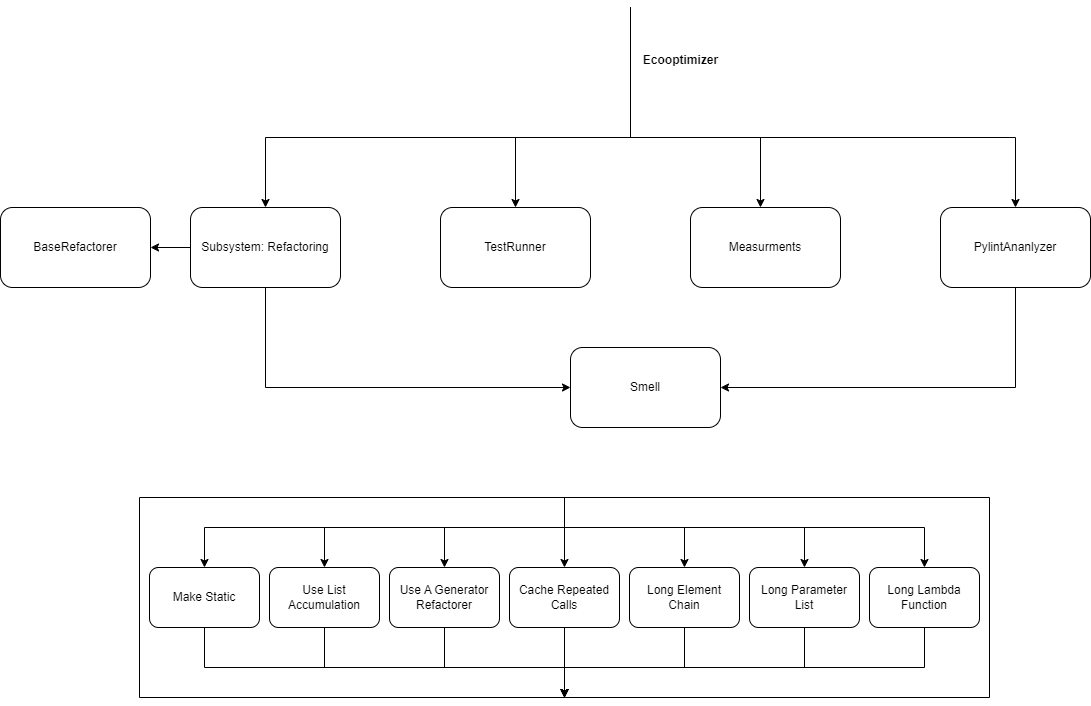
\includegraphics[width=\textwidth]{../../Images/use_hierarchy_modules.png}
\caption{Use hierarchy among modules}
\label{FigUH}
\end{figure}

%\section*{References}

\section{User Interfaces}

\wss{Design of user interface for software and hardware.  Attach an appendix if
needed. Drawings, Sketches, Figma}

\section{Design of Communication Protocols}

\wss{If appropriate}

\section{Timeline}

All code and corresponding documentation was aimed to be completed before Jan 6th our Demo date for our supervisor.

\begin{table}[h!]
  \centering
  \caption{Timeline}
  \begin{tabular}{|l|l|l|}
  \hline
  \textbf{Module Name} & \textbf{Team Member}        & \textbf{Due Date} \\ \hline
  Base Refactorer                     & Sevhena Walker              & Jan 6, 2025    \\ \hline
  Complex List Comprehension          & Nivetha Kuruparan              & Jan 6, 2025    \\ \hline
  Long Element Chain                  & Ayushi Amin              & Jan 6, 2025     \\ \hline
  Long Lambda Function                & Mya Hussain              & Jan 6, 2025     \\ \hline
  Long Message Chain                  & Mya Hussain              & Jan 6, 2025     \\ \hline
  Member Ignoring Method              & Sevhena Walker             & Jan 6, 2025     \\ \hline
  Repeated Calls                      & Nivetha Kuruparan               & Jan 6, 2025     \\ \hline
  String Concatenation in Loop        & Sevhena Walker              & Jan 6, 2025     \\ \hline
  Long Parameter List                 & Tanveer Brar              & Jan 6, 2025     \\ \hline
  Smell                               & All             & Jan 31, 2025    \\ \hline
  Analyzers                           & All            & Jan 31, 2025      \\ \hline
  Measurements                        & All          & Jan 31, 2025      \\ \hline
  Testing Functionality               & All           & Jan 31, 2025      \\ \hline
  \end{tabular}
  \end{table}
  

\bibliographystyle {plainnat}
\bibliography{../../../refs/References}

\newpage{}

\end{document}